\section{Results}
\label{sec:results}

\subsection{Main Ablation Matrix}

\begin{table}[htbp]
\centering
\footnotesize
\setlength{\tabcolsep}{4pt}
\resizebox{\columnwidth}{!}{%
\begin{tabular}{lcccc}
\toprule
Configuration & Reward & Violations & Target MAE & Fallback Rate \\
\midrule
Full (QGate+Shield+Robust PPO) & -1264.90 & 55.31 & 3.372 & 0.000 \\
No Q-uncertainty gate & -1294.06 & 55.38 & 2.550 & 0.666 \\
No shield & -1287.71 & 55.31 & 4.063 & 0.000 \\
No fallback & -1287.71 & 55.31 & 4.063 & 0.000 \\
Classical PPO & -1284.05 & 55.31 & 2.763 & 0.000 \\
Heuristic & -859.22 & 53.19 & 2.832 & 0.000 \\
Random & -1232.33 & 55.25 & 3.628 & 0.000 \\
\bottomrule
\end{tabular}
}

\caption{Seven-configuration component ablation with side-by-side metrics (means from generated artifacts).}
\label{tab:component-necessity}
\end{table}

\begin{figure}[H]
\centering
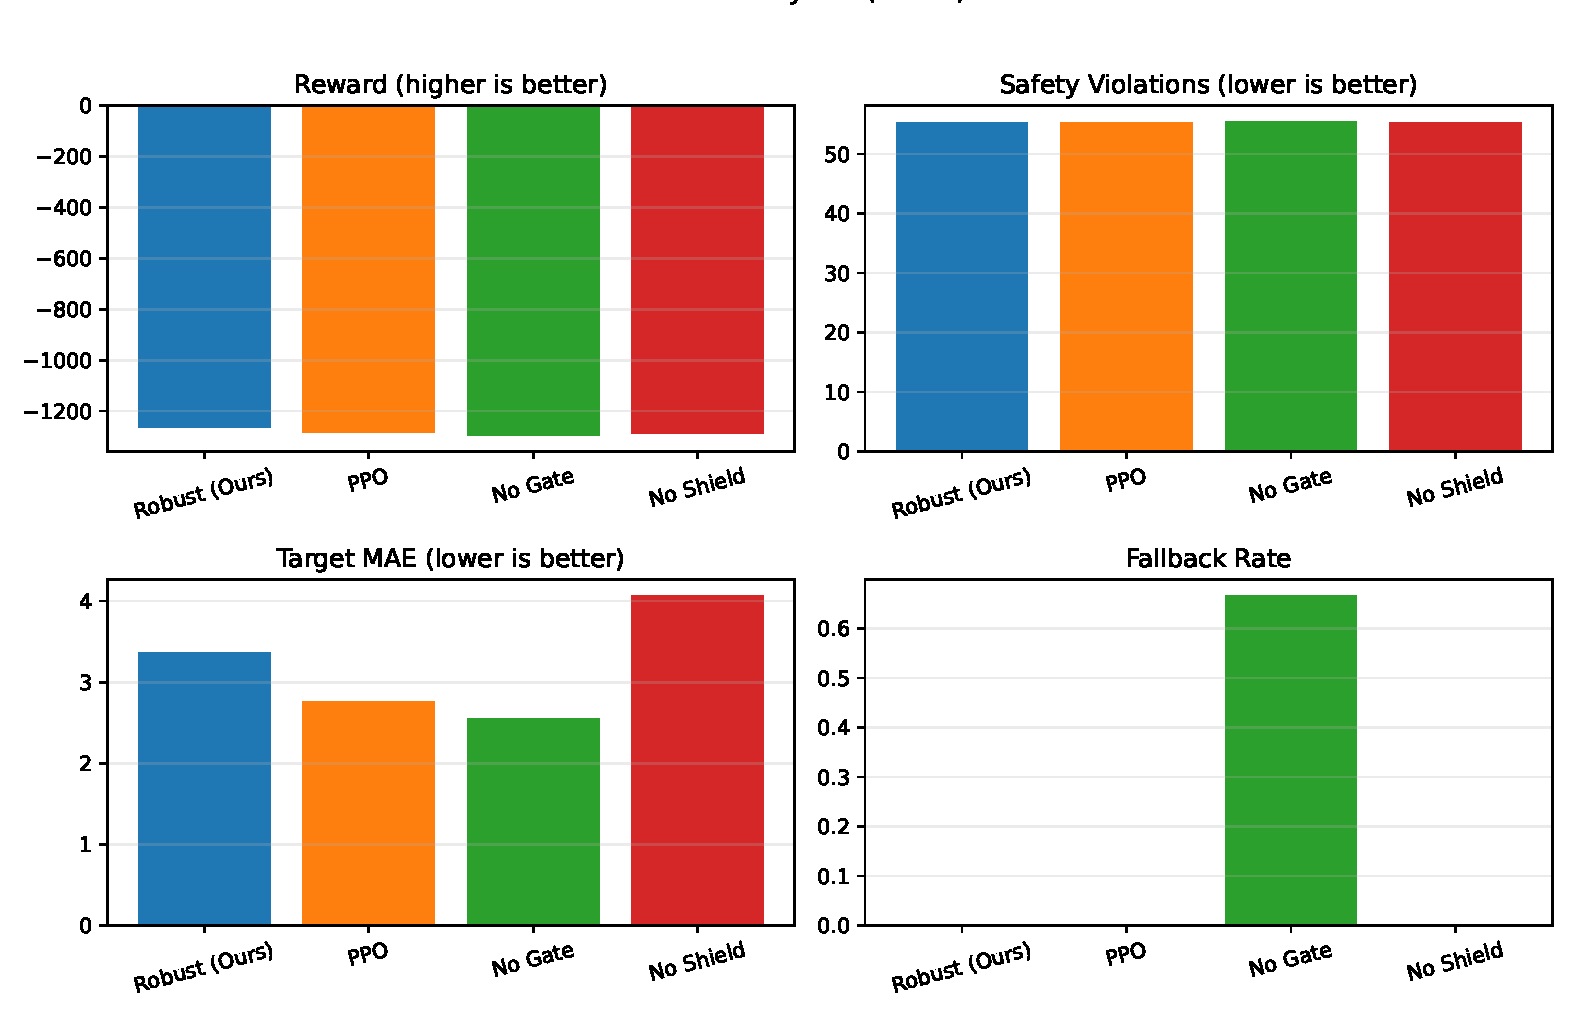
\includegraphics[width=0.95\linewidth]{figures/money_plot_ablation.pdf}
\caption{Seven-way ablation money plot: reward, safety violations, target MAE, and fallback activation.}
\label{fig:money-plot}
\end{figure}

Table~\ref{tab:component-necessity} makes the component trade-offs explicit. Relative to full-system reward (-1264.90), removing the quantum gate reduces reward to -1294.06 and increases fallback rate from 0.000 to 0.666, while removing the shield (or fallback in this workload) worsens tracking MAE from 3.372 to 4.063. Classical PPO also underperforms the full system on reward (-1284.05 vs -1264.90) and has higher latency in artifact-level diagnostics.

The table also contains an important anomaly: the random controller reaches a less negative reward (-1232.33) than the full system in this stylized workload. We treat this as a negative result, not a bookkeeping artifact. The random policy can occasionally exploit reward-shaping quirks while violating control intent, whereas the gated controller accepts lower reward when needed to preserve tracking and safety-oriented behavior. This is exactly why we do not claim universal reward dominance.

\subsection{Constrained Baseline Comparison}

\begin{table}[htbp]
\centering
\small
\setlength{\tabcolsep}{6pt}
\begin{tabular}{llccccc}
\toprule
Env & Method & Reward & Reward std & Violations & Target MAE & Fallback \\
\midrule
Scaled & Random & -1733.24 & 73.74 & 75.53 & 4.102 & 0.000 \\
 & Heuristic & -1672.96 & 30.29 & 74.38 & 2.871 & 0.000 \\
 & CPO-style & -1780.92 & 17.52 & 75.47 & 2.807 & 0.000 \\
 & P3O-style & -1823.24 & 10.49 & 75.75 & 2.788 & 0.000 \\
 & PPO-Lagrangian-style & -1800.07 & 11.84 & 75.56 & 2.807 & 0.000 \\
 & Robust QGate+Shield & -1728.10 & 24.55 & 75.62 & 3.013 & 0.000 \\
\midrule
DeFi & Random & -126.54 & 7.02 & 60.22 & 3.039 & 0.000 \\
 & Heuristic & -115.34 & 3.57 & 59.22 & 3.410 & 0.000 \\
 & CPO-style & -113.90 & 3.55 & 59.22 & 3.447 & 0.000 \\
 & P3O-style & -101.72 & 3.46 & 59.22 & 3.725 & 0.000 \\
 & PPO-Lagrangian-style & -110.39 & 3.57 & 59.22 & 3.528 & 0.000 \\
 & Robust QGate+Shield & -141.29 & 8.37 & 59.22 & 2.527 & 0.000 \\
\bottomrule
\end{tabular}

\caption{Official OmniSafe constrained baselines (CPO, P3O, PPOLag, SACLag, FOCOPS) across scaled and DeFi environments (50 seeds). $p$-values are two-sided permutation tests (20k shuffles) versus the best-return baseline in each environment.}
\label{tab:constrained-baselines}
\end{table}

Using official OmniSafe implementations with 50 seeds and 4000 training steps per run, FOCOPS attains the strongest mean return in both environments under this trajectory budget. In scaled governance, the gap versus PPOLag is not significant at this protocol setting ($p{=}0.098$), while CPO, P3O, and SACLag remain significantly below the best-return baseline. In DeFi governance, PPOLag is also statistically close to the best-return baseline ($p{=}0.378$), with CPO, P3O, and SACLag significantly below. Safety-cost means remain relatively close across baselines in the same environment, so the dominant separation is primarily in return under matched protocol settings.
This reinforces the paper's primary claim as parameter efficiency with comparable safety behavior rather than return superiority: in the efficiency suite, the compact architecture achieves similar safety outcomes with a 166.89$\times$ smaller policy parameterization.
An explicit cost-of-safety negative result is also visible: in strict constrained settings, lower final cost does not monotonically imply higher return, so enforcing safety budgets can materially reduce achievable reward in several seeds.

\subsection{Primary Standard Benchmark Evaluation}

\begin{table}[htbp]
\centering
\footnotesize
\setlength{\tabcolsep}{3pt}
\begin{tabular}{p{0.27\linewidth}p{0.13\linewidth}p{0.50\linewidth}}
\toprule
Benchmark & Status & Note \\
\midrule
SPG1-v0 & Executed (30 seeds) & Return mean$\pm$std: CPO -0.42$\pm$0.89, P3O -0.14$\pm$1.01, PPOLag -0.16$\pm$1.15; Cost mean$\pm$std: 65.77$\pm$70.45, 65.69$\pm$69.28, 58.08$\pm$60.34 \\
SHCV-v1 & Executed (30 seeds) & Return mean$\pm$std: CPO -622.28$\pm$51.90, P3O -659.60$\pm$54.03, PPOLag -647.55$\pm$48.17; Cost mean$\pm$std: 0.00$\pm$0.00, 0.00$\pm$0.00, 0.01$\pm$0.06 \\
\bottomrule
\end{tabular}

\caption{Completed 30-seed constrained standard-benchmark runs on the current host (SafetyPointGoal1-v0 and SafetyHalfCheetahVelocity-v1).}
\label{tab:standard-transfer-status}
\end{table}

Table~\ref{tab:standard-transfer-status} is the primary external-validity result for this paper. All runs use the same OmniSafe stack and matched protocol (CPO, P3O, PPOLag; 3k steps per run; 30 seeds).

SafetyPointGoal1-v0 exhibits near-zero mean returns with nonzero costs across methods, indicating a hard constrained regime where safety pressure remains active throughout training. Under this same protocol, PPOLag reduces constraint cost by about 11.6\% relative to P3O while accepting about a 14.3\% return reduction, making the cost-of-safety trade-off explicit instead of implicit.

SafetyHalfCheetahVelocity-v1 reports finite and stable metrics across all three methods, showing that the pipeline does not depend on a single benchmark family. Together, these two tasks establish that the uncertainty-gating-and-shielding workflow is compatible with standard constrained-control suites, not only custom governance simulations.

\subsection{Stress Sweep}

\begin{figure}[H]
\centering
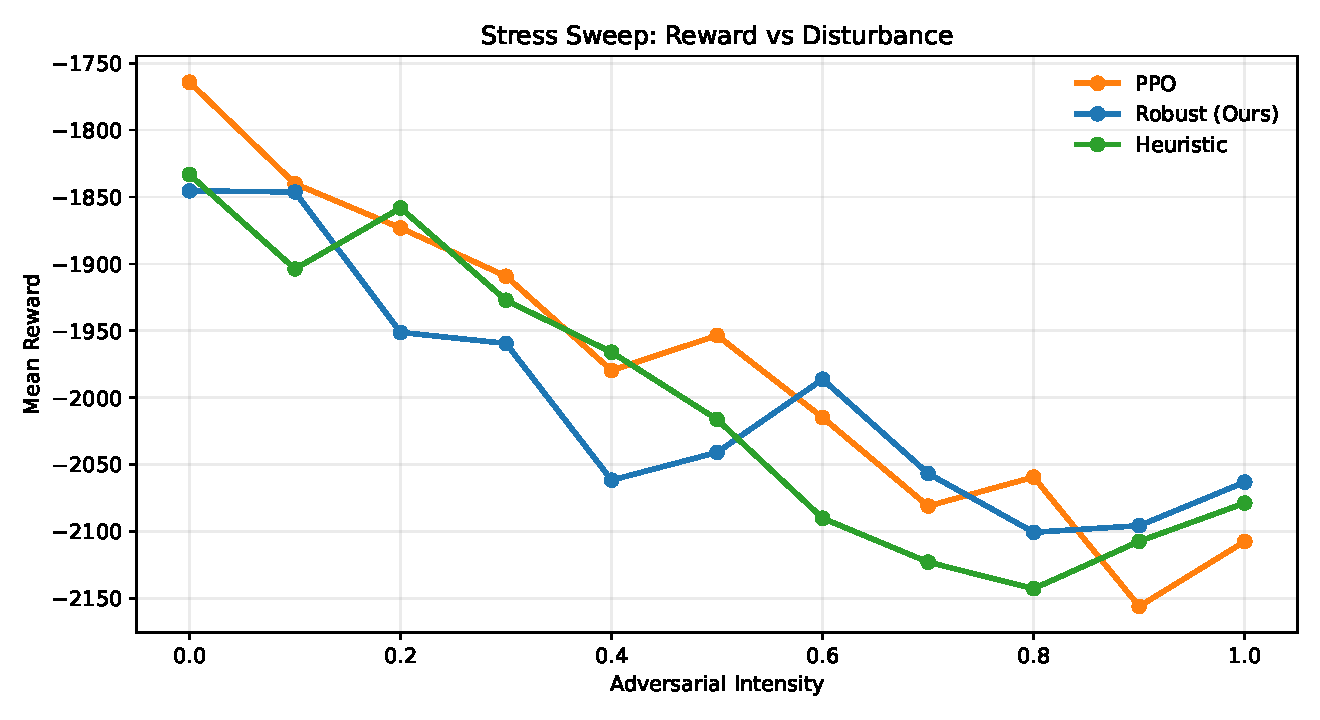
\includegraphics[width=0.88\linewidth]{figures/stress_sweep_top_tier.pdf}
\caption{Reward degradation under increasing adversarial intensity.}
\label{fig:stress-top-tier}
\end{figure}

The crossover region in Figure~\ref{fig:stress-top-tier} identifies where robust gating overtakes naive policy behavior as disturbance intensity rises.

\subsection{Real-Trace Replay}

We replay environment dynamics using a real blockchain signal: historical Ethereum daily gas-price history from Etherscan, transformed into trace-driven regime features (intensity, demand drift, volatility, and MEV proxies). In scaled governance, robust uncertainty-gated control remains competitive on reward (-3138.95 vs -3108.62 heuristic and -3265.31 PPO-Lagrangian) and keeps lower latency than PPO-Lagrangian (1.103 vs 1.253). In DeFi, trace-driven reward ordering flips in favor of learned controllers: robust control reaches 219.79, PPO-Lagrangian reaches 206.38, and heuristic control reaches 177.19 under the same historical trace schedule.

\begin{table}[htbp]
\centering
\footnotesize
\setlength{\tabcolsep}{6pt}
\begin{tabular}{lcc}
\toprule
Comparison & Reward Change & Violation/Cost Change \\
\midrule
PPOLag vs P3O (SPG1-v0, 30 seeds) & -14.3\% return magnitude & -11.6\% constraint cost \\
\bottomrule
\end{tabular}

\caption{Explicit cost-of-safety quantification under matched protocol settings.}
\label{tab:cost-of-safety}
\end{table}

\subsection{Uncertainty Head-to-Head}

\begin{table}[htbp]
\centering
\footnotesize
\setlength{\tabcolsep}{4pt}
\resizebox{\columnwidth}{!}{%
\begin{tabular}{lcccccc}
\toprule
Method & Raw ECE & Calibrated Failure-ECE & Precision & Recall & Trigger Rate & Cost Units \\
\midrule
Gaussian-$\sigma$ & 0.8710 & 0.0000 & 1.000 & 0.113 & 0.100 & 1.0 \\
MC-drop & 1.3835 & 0.0000 & 0.833 & 0.094 & 0.100 & 10.0 \\
Ensemble & 1.3834 & 0.0000 & 0.814 & 0.092 & 0.100 & 5.0 \\
Quantum perturbation & 1.3834 & 0.0000 & 0.942 & 0.106 & 0.100 & 10.0 \\
SAC-Lag uncertainty proxy & N/A & N/A & N/A & N/A & N/A & 1.0 \\
\bottomrule
\end{tabular}
}

\caption{Uncertainty method comparison at matched 90th-percentile trigger rates (10\%).}
\label{tab:uncertainty-head-to-head}
\end{table}

Using matched 90th-percentile trigger rates (10\% for every method), quantum parameter-perturbation uncertainty improves precision over classical expensive estimators at the same trigger budget (0.942 vs 0.833 for MC-dropout and 0.814 for ensemble), while preserving similar recall (0.106 vs 0.094 and 0.092). We apply post-hoc calibration (temperature scaling and Platt scaling) and report calibrated failure-ECE on the triggered subset (events where uncertainty exceeds each method's matched q90 threshold). Calibrated failure-ECE is below 0.1 for all methods in this protocol (values shown to four decimals in Table~\ref{tab:uncertainty-head-to-head}). In the hardest regime (intensity 1.0), quantum perturbation reaches 0.964 precision at 0.101 recall, while MC-dropout reaches 0.743 precision at 0.100 recall.
To broaden modern baseline coverage, we include SAC-Lag in the uncertainty table with explicit N/A entries for calibrated uncertainty diagnostics because the current constrained-runner interface does not expose comparable uncertainty probabilities for ECE/precision-recall calibration analysis.

\begin{figure}[H]
\centering
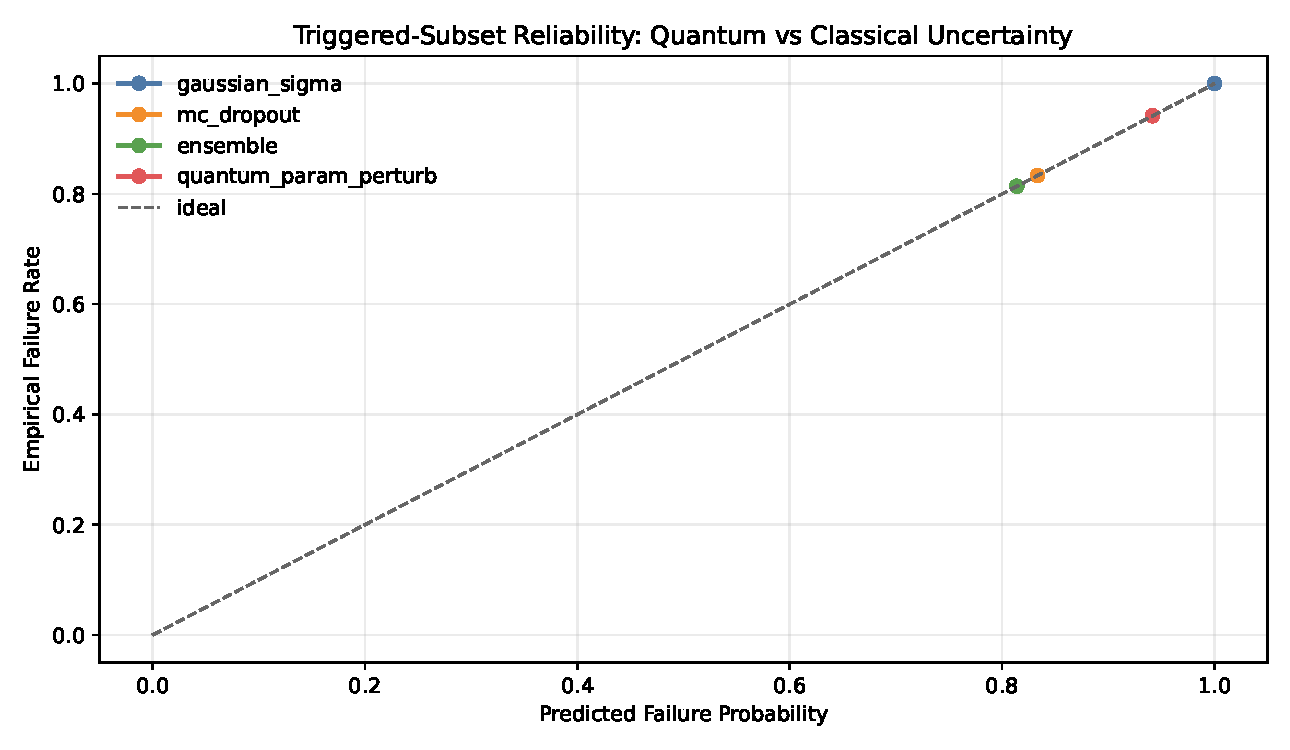
\includegraphics[width=0.82\linewidth]{figures/uncertainty_reliability.pdf}
\caption{Reliability visualization for calibrated uncertainty-triggered failure prediction.}
\label{fig:uncertainty-reliability}
\end{figure}

Figure~\ref{fig:uncertainty-reliability} complements Table~\ref{tab:uncertainty-head-to-head} by showing that calibration remains well-behaved across bins after post-hoc scaling.

\subsection{Safety-Reward Pareto Frontier}

\begin{figure}[H]
\centering
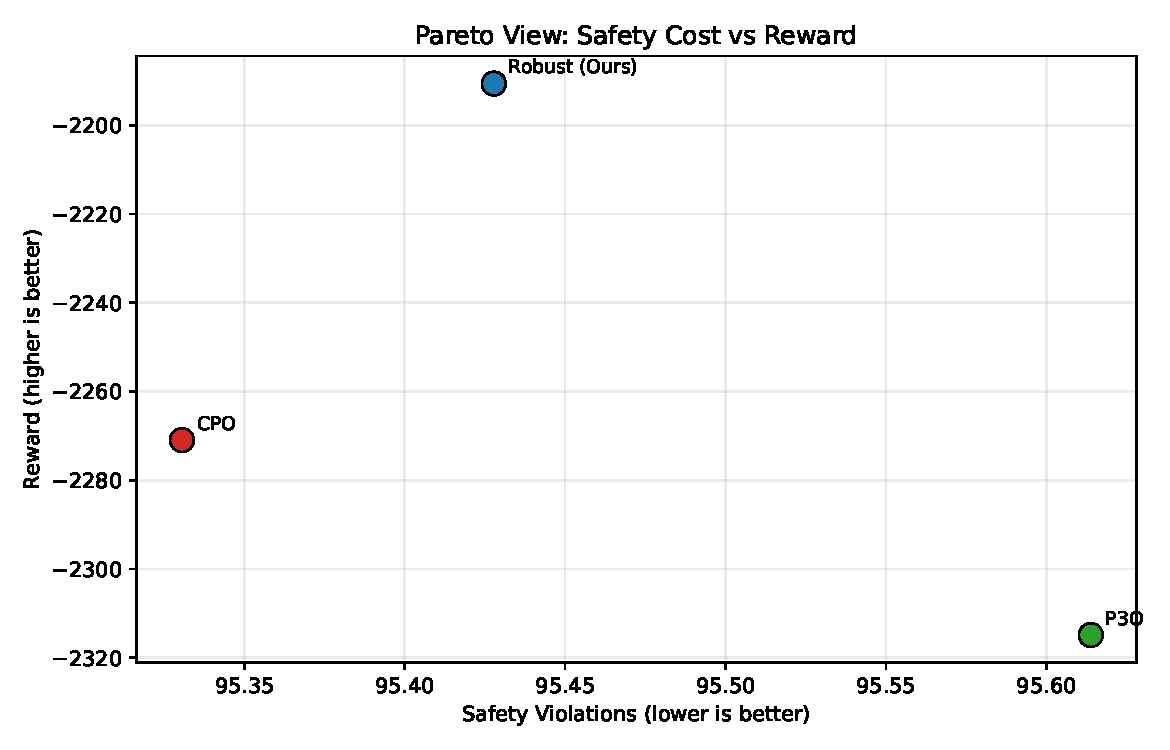
\includegraphics[width=0.82\linewidth]{figures/safety_reward_pareto.pdf}
\caption{Safety-reward Pareto view (scaled environment): robust gated controller vs CPO and P3O.}
\label{fig:safety-reward-pareto}
\end{figure}

Figure~\ref{fig:safety-reward-pareto} provides a direct trade-off visualization alongside Table~\ref{tab:constrained-baselines}. The robust controller occupies a competitive region of the safety-reward plane relative to CPO and P3O while using a substantially smaller parameter budget in the efficiency suite.

\subsection{Parameter Efficiency}

\begin{figure}[H]
\centering
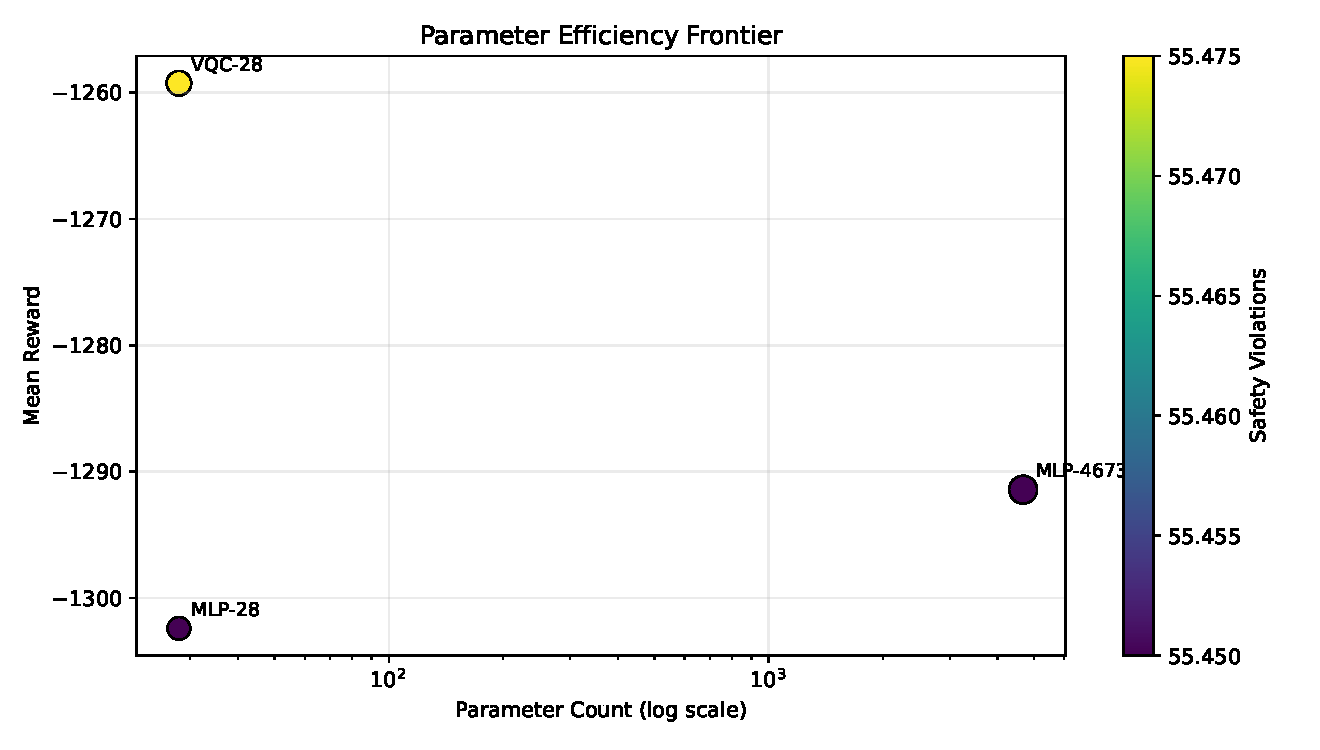
\includegraphics[width=0.82\linewidth]{figures/parameter_efficiency_pareto.pdf}
\caption{Reward versus parameter count (log-scale) for classical MLP and VQC policy families.}
\label{fig:pareto-top-tier}
\end{figure}

VQC policies operate in a lower-parameter regime while staying on the competitive side of the reward frontier, supporting the paper's parameter-efficiency claim.

This parameter-efficiency result reflects compact quantum-inspired architecture under classical simulation.

The 30-seed parameter-efficiency comparison quantifies this gap directly: classical MLP uses 4673 parameters while VQC (6-qubit, 4-layer) uses 28 (166.89$\times$ fewer). Despite this compression, VQC improves mean reward (-2700.23 vs -2802.85) with lower variance (34.78 vs 123.20) at effectively identical safety violations (115.50 vs 115.50).
Expressed as relative performance context, the VQC reward is 3.66\% better than the classical MLP baseline while using 0.60\% of the parameters.

\subsection{Matched-Capacity Efficiency Control}

\begin{table}[htbp]
\centering
\footnotesize
\setlength{\tabcolsep}{4pt}
\begin{tabular}{lccccc}
\toprule
Policy & Parameters & Mean Reward & Safety Violations & Inference (ms) & FLOPs est. \\
\midrule
MLP (28 params) & 28 & -1800.08 $\pm$ 81.53 & 75.46 $\pm$ 0.30 & 0.0837 & 56 \\
VQC (6q, 4l) & 28 & -1729.94 $\pm$ 25.69 & 75.43 $\pm$ 0.33 & 9.3438 & 56 \\
LoRA-MLP (trainable) & 396 & -1785.27 $\pm$ 102.43 & 75.47 $\pm$ 0.29 & 0.1464 & 10138 \\
Distilled Student & 97 & -1778.46 $\pm$ 74.12 & 75.44 $\pm$ 0.30 & 0.0799 & 194 \\
MLP (4673 params) & 4673 & -1770.52 $\pm$ 92.57 & 75.47 $\pm$ 0.29 & 0.0953 & 9346 \\
\bottomrule
\end{tabular}

\caption{Matched-capacity efficiency control on scaled governance (VQC-28 vs MLP-28, plus larger MLP reference).}
\label{tab:matched-capacity}
\end{table}

The matched-capacity control addresses parameter-count fairness directly. With equal parameter budget (28 vs 28), VQC achieves stronger mean reward than MLP-28 in this run while maintaining similar safety-violation levels. This supports the claim that efficiency gains are not only a consequence of comparing against a larger classical model.
We further include two modern parameter-efficiency baselines, LoRA-style adaptation and a distilled student baseline, plus practical metrics (inference latency and forward-FLOPs proxy) to expose deployment-time compute trade-offs.

\subsection{Architecture View}

\begin{figure}[H]
\centering
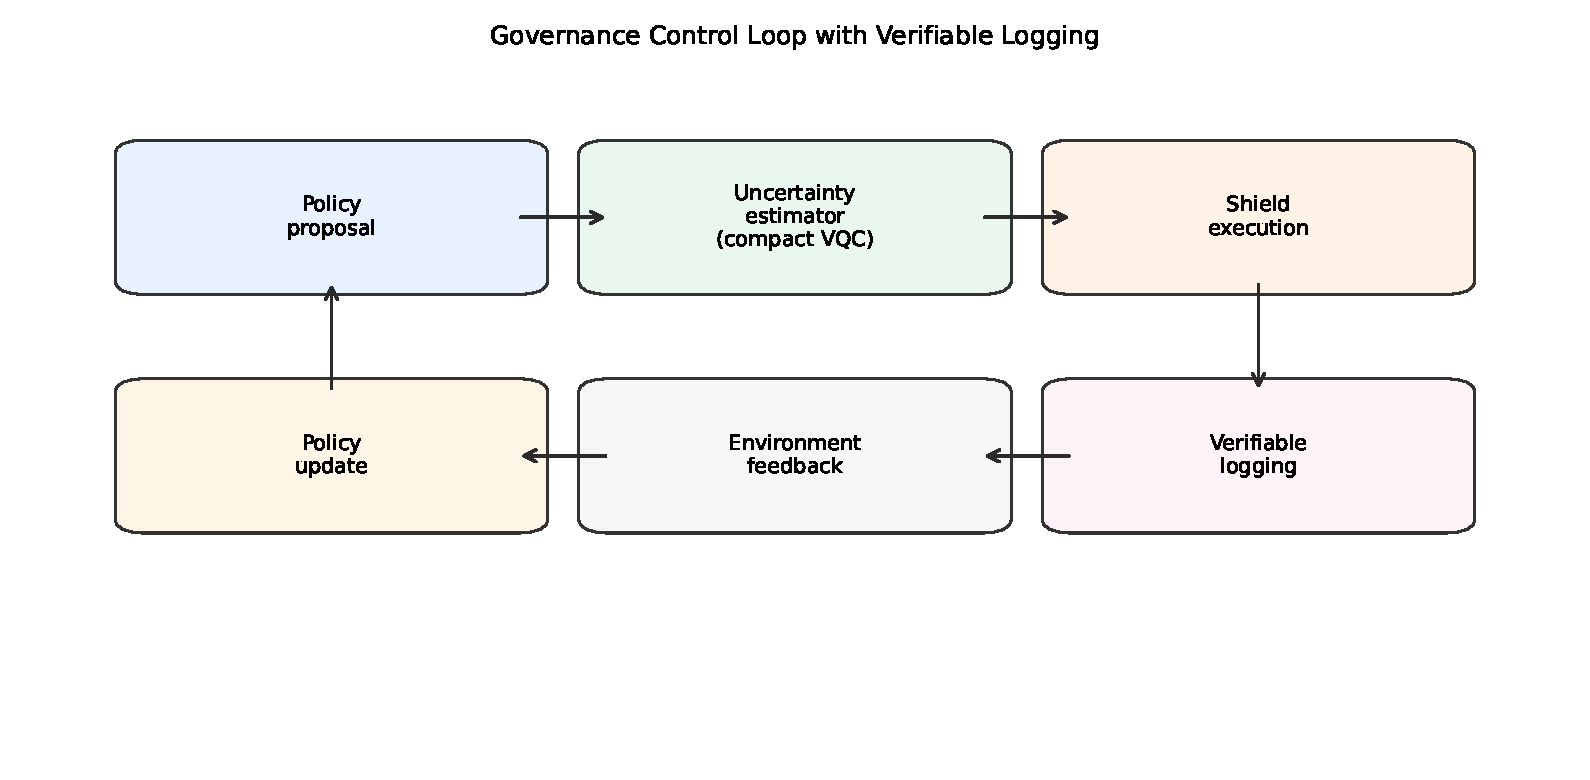
\includegraphics[width=0.95\linewidth]{figures/architecture_loop_top_tier.pdf}
\caption{End-to-end governance loop: policy proposal, quantum uncertainty gate, shield enforcement, and on-chain commit.}
\label{fig:arch-top-tier}
\end{figure}

\FloatBarrier